\chapter{Experimental Evaluation}
\label{chpt:6}
\paragraph{}
In this chapter we present the experiments that we performed to evaluate our system. We analyze the results, and present some problems of our approach.


Using our multilingual relation extraction dataset \textbf{X-WikiRE}, we evaluate two types of settings:
\begin{itemize}
    \item \textbf{UnENT} in which the model is tested on unseen entities as in traditional relation extraction systems, and the zero-shot setting
    \item  \textbf{UnREL} in which the model performance are evaluated on unseen relations (the entities may or may not been seen at training).
\end{itemize}

Our goal is to answer three different questions: \begin{enumerate*}[a) , font=\bfseries]
    \item how well relation extraction models can be transferred across different languages?
    \item can the variance in the number of relations examples between languages help  build more robust relation extraction models?
    \item can a jointly trained model that performs RE on multiple languages perform equally or better than the monolingual trained version? 
\end{enumerate*}

\section{Experimental Setting}
\subsection{Metrics}
\paragraph{}
We use the same evaluation methodology as ~\cite{levy2017zero}. We compute the precision, recall, and F1-score by comparing the spans of the answers predicted by the model with the ground truth answer span. The measure does not take in consideration the word order and punctuation but articles are not removed from the evaluation as separating them from entities is not as trivial for other languages as it is for English.

\begin{equation}
    precision = \frac{\textit{\# of matching content words}}{\textit{\# of content words in predicted answer}}
\label{eq:precision}
\end{equation}


\begin{equation}
    recall = \frac{\textit{\# of matching content words}}{\textit{\# of content words in ground truth answer}}
\label{eq:recall}
\end{equation}


\begin{equation}
    \textit{F1-score} = 2 * \frac{precison * recall}{precision + recall}
\label{eq:f1}
\end{equation}

\subsection{Hyperparameters}
\paragraph{}
In all experiments, models were trained for five epochs with a learning rate of $1.0$ using Adam \citep{kingma2014adam} as optimizer with $\beta_1 = 0.01, \beta_2 = 0.999$, $\epsilon = 1e - 8$. For finetuning in the cross-lingual transfer experiments, the learning rate was lowered to $0.001$ to prevent forgetting and a maximum of $30$ iterations over the small target language training set were performed with model selection using the target language development set F1-score. 

The embeddings used are from the multilingual fastText, except when comparing against BERT and when confronting on the dataset of \cite{levy2017zero}, where we use GloVe to maintain the compatibility of results. 

% All monolingual models' word embeddings were initialised using fastText embeddings, except for the comparison experiments described in sub-section \ref{subsec:comparisonbert} and in \ref{subsec:comparison} where GloVe \citep{pennington2014glove} was used for comparability with \cite{levy2017zero}.

\section{Word Representation}
\paragraph{}
We compared the two multilingual word embedding models presented in Section~\ref{sec:w_e} to find which of them is the best solution for our task. To compare these two solution we used the \textit{ Cross-lingual Model Transfer} setup described in Section~\ref{sec:xlingual}. The model is first trained using 1M examples on a high resource language (English) then fine-tuning on the target language is performed. The fine-tuning is performed with different amount of examples, the settings are: zero-shot (0 examples), 1K, 2K, 5K, and 10K. Table~\ref{table:resultsunentcompare} shows the results for our model in the \textbf{UnENT} scenario using both multilingual BERT and fastText. As we can see, BERT performs poorly compared to fastText in every language and almost for each of the fine-tuning settings. 

\begin{table}[h!]
\centering

\begin{adjustbox}{width=0.6\columnwidth}

\begin{tabular}{c|r|c|c|c|c|c|c}
\toprule
\multirow{2}{*}{} & \multicolumn{1}{c|}{\multirow{2}{*}{Setting}} & \multicolumn{3}{c|}{BERT} & \multicolumn{3}{c}{fastText} & 
 & \multicolumn{1}{c|}{} & P & R & F1 & P & R & F1 \\ \hline
\multirow{5}{*}{\rotatebox[origin=c]{90}{EN-IT}} & 0 & 9.76 & 11.84 & \textbf{10.70} & 54.86 & 2.31 & 4.44 \\ %& - & - & - \\ %\cline{2-8} 
 & 1K & 64.15 & 50.08 & 56.25 & 69.25 & 59.53 & \textbf{64.02} \\ %& 00.00 & 00.00 & 00.00 \\ %\cline{2-8} 
 & 2K & 70.89 & 57.12 & 63.26 & 80.78 & 68.89 & \textbf{74.37} \\ %& 00.00 & 00.00 & 00.00 \\ %\cline{2-8} 
 & 5K & 79.85 & 68.33 & 73.64 & 83.77 & 81.90 & \textbf{82.82} \\ %& 00.00 & 00.00 & 00.00 \\ %\cline{2-8} 
 & 10K & 83.39 & 76.97 & 80.06 & 84.43 & 82.50 & \textbf{83.45} \\ \hline \hline %& 00.00 & 00.00 & 00.00 \\ 
%& %Full & - & - & - & - & - & - & 88.69 & 88.10 & 88.39 \\   
\multirow{5}{*}{\rotatebox[origin=c]{90}{EN-ES}} & 0 & 10.22 & 3.75 & 5.49 & 28.98 & 11.22 & \textbf{16.17} \\ %& - & - & - \\ %\cline{2-8}
 & 1K & 55.19 & 35.19 & 42.97 & 67.56 & 64.08 & \textbf{65.78} \\ %& 00.00 & 00.00 & 00.00 \\ %\cline{2-8} 
 & 2K & 68.43 & 50.36 & 58.02 & 74.45 & 72.73 & \textbf{73.58} \\ %& 00.00 & 00.00 & 00.00 \\ %\cline{2-8} 
 & 5K & 72.65 & 63.97 & 68.04 & 79.23 & 74.03 & \textbf{76.54} \\ %& 00.00 & 00.00 & 00.00 \\ %\cline{2-8} 
 & 10K & 79.76 & 65.06 & 71.66 & 79.27 & 76.76 & \textbf{77.99} \\ \hline \hline %& 00.00 & 00.00 & 00.00 \\ 
 %& Full & - & - & - & - & - & - & 81.79 & 85.02 & 83.37 \\\hline \hline
\multirow{5}{*}{\rotatebox[origin=c]{90}{EN-FR}} & 0 & 23.72 & 13.77 & \textbf{17.42} & 49.56 & 9.03 & 15.28 \\ %& - & - & - \\ %\cline{2-8} 
 & 1K & 53.81 & 35.38 & 42.69 & 69.88 & 61.93 & \textbf{65.67} \\ %& 00.00 & 00.00 & 00.00 \\ %\cline{2-8} 
 & 2K & 67.51 & 52.74 & 59.21 & 77.30 & 63.37 & \textbf{69.64} \\ % & 00.00 & 00.00 & 00.00 \\ %\cline{2-8} 
 & 5K & 70.98 & 66.16 & 68.49 & 76.35 & 69.11 & \textbf{72.55} \\ % & 00.00 & 00.00 & 00.00 \\ %\cline{2-8} 
 & 10K & 78.67 & 67.11 & 72.43 & 80.78 & 68.52 & \textbf{74.15} \\ \hline \hline % & 00.00 & 00.00 & 00.00 \\ 
% & Full & - & - & - & - & - & - & 82.36 & 74.16 & 78.05 \\\hline \hline
\multirow{5}{*}{\rotatebox[origin=c]{90}{EN-DE}} & 0 & 3.33 & 2.52 & 2.87 & 21.00 & 10.60 & \textbf{14.09} \\ %& - & - & - \\ %\cline{2-8}
 & 1K & 50.84 & 62.35 & 56.01 & 55.84 & 70.91 & \textbf{62.47} \\ %& 00.00 & 00.00 & 00.00 \\ %\cline{2-8} 
 & 2K & 58.46 & 65.96 & 61.99 & 56.67 & 75.13 & \textbf{64.60} \\ % & 00.00 & 00.00 & 00.00 \\ %\cline{2-8} 
 & 5K & 61.37 & 71.75 & 66.16 & 68.00 & 76.24 & \textbf{71.88} \\ %& 00.00 & 00.00 & 00.00 \\ %\cline{2-8} 
 & 10K & 66.65 & 74.66 & 70.43 & 66.89 & 78.37 & \textbf{72.17} \\ % & 00.00 & 00.00 & 00.00 \\ %\hline
 %& Full & - & - & - & - & - & - & 75.85 & 88.21 & 81.57 \\
\bottomrule
\end{tabular}
\centering
\end{adjustbox}
\caption{Precision, Recall and F1-scores for \textbf{UnENT} comparing scores using BERT and fastText multilingual embeddings.}
\label{table:resultsunentcompare}

\end{table}


A reason of this can be the high difference in word coverage. As shown in Table \ref{tab:lang_model_coverage}, the vocabulary coverage for the contexts and questions is double for all languages for fastText compared to BERT. This is caused by the disparity in the number of words in the vocabulary of the embeddings. BERT has only 120K tokens for 104 languages, while fastText's vocabulary contains around 100K tokens for each language.  

\begin{table}[h!]
  \centering
  \begin{adjustbox}{width=0.6\columnwidth}
    \begin{tabular}{c|cc|cc}
    \toprule
          & \multicolumn{2}{c|}{BERT} & \multicolumn{2}{c}{fastText} \\
    \midrule
    \multicolumn{1}{l|}{Lang.} & Context & Question & Context & Question \\
    \midrule
    IT    & 24\%  & 35\%  & 64\%  & 71\%  \\
    FR    & 25\%  & 36\%  & 67\%  & 73\%  \\
    ES    & 24\%  & 37\%  & 65\%  & 73\%  \\
    DE    & 22\%  & 34\%  & 56\%  & 64\%  \\
    EN    & 30\%  & 37\%  & 63\%  & 71\%  \\
    \bottomrule
    \end{tabular}%
  \end{adjustbox}
  \caption{Vocabulary coverage for multilingual BERT and fastText.}
  \label{tab:lang_model_coverage}%

\end{table}%

\newpage

\section{Transfer Setups}
\paragraph{}
We perform experiments of the two previously described architectures to see how well each scenario perform in different types of multilingual and cross-lingual transfer. We also present the results for the monolingual setup, and use it as a comparison for the multilingual models. 


\subsection{Monolingual}
\paragraph{}
We train a model for each language on the full monolingual training set (1 million of instances), the model will be used as a comparison for the multilingual and the cross-lingual transfer models. Table~\ref{table:baseline} presents the results obtained for both the \textbf{UnENT} and \textbf{UnREL} scenarios. The monolingual should be seen as a ceiling, as the other models will be trained with less data.

\begin{table}[ht!]
\fontsize{10}{10}\selectfont
%\begin{adjustbox}{width=\textwidth}
  \centering
  %\scriptsize
    \begin{tabular}{c|c|c|c}
    \toprule
    {Lang.} & & {UnENT} & {UnREL} \\

     \midrule
     
     \multirow{3}{*}{EN} & P  &    74.09            & 46.75 \\
                         & R  &    85.35            & 25.32 \\
                         & F1 &    79.32            & 32.78 \\

     \midrule
     \multirow{3}{*}{ES} & P  &    81.79            & 49.77 \\
                         & R  &    {85.02}          & 27.69 \\
                         & F1 &    83.37            & 34.54 \\

     \midrule
     \multirow{3}{*}{IT} & P  &    {88.69}   & 47.09 \\
                         & R  &    {88.10}   & 29.45 \\
                         & F1 &    {88.39}   & 35.62 \\

     \midrule
     \multirow{3}{*}{FR} & P  &    82.36            & 42.93 \\
                         & R  &    74.16            & 25.73 \\
                         & F1 &    78.05            & 31.78 \\

     \midrule
     \multirow{3}{*}{DE} & P  &    {75.85}   & 41.94 \\
                         & R  &    {88.21}   & 24.38 \\
                         & F1 &    {81.57}   & 30.82 \\

    %\multirow{3}{*}{\rotatebox[origin=c]{90}{UnREL}} & LV & 43.56 / 36.45 / 39.61 & - / -  / - & - / - / - & - / - / - & - / - / - & - / - / - \\
    %     & Mono. & 56.53 / 44.74 / 49.85 & 46.75 / 25.32 / 32.78 &  - / -  / - & - / -  / -  & - / -  / -  &  - / -  / -  \\
    %     & Multi. & - / -  / -    &  - / -  / -     &   - / -  / -    &  - / -  / -     &    - / -  / -   &   \\
    \bottomrule
    \end{tabular}
    %\end{adjustbox}
      \caption{Precision, Recall, and F1-scores for the monolingual baseline for all languages in the \textbf{UnENT} and \textbf{UnREL} setup.}
  \label{table:baseline}
\end{table}




\subsection{Cross-lingual Model Transfer}
\paragraph{}
In this set of experiments, we test how well RE models can be transferred from a source language with a large number of training examples to target languages with no or minimal training data (question \textbf{a}). 

In the \textbf{UnENT} experiments, we construct pairwise parallel test and development sets between English and each of the languages, meaning that the entities that are in the English and the target train/dev set are non present in the target test set. Then an English relation extraction model, built  on  top  of  the  multilingual representations, is trained on a full English training set (1 million instances). A similar approach is followed also for the \textbf{UnREL} scenario, in this case the train/dev sets do not contain any relation that is in the target's language test set.

The results presented in Table~\ref{tab:lang_model_coverage} are for the cross-lingual transfer \textbf{UnENT} experiments. While it is clear that the models suffer from rather low recall when no fine-tuning is performed,  the  results  show considerable  improvements when performing fine-tuning with just 1000 target language examples. When using 10K target language examples, it is possible to nearly match the performance of a model trained on the full target language monolingual training set. In Figure~\ref{fig:UnEntF1}, we can have better view of the performances when using fastText.

\begin{figure*}[h!]
\centering
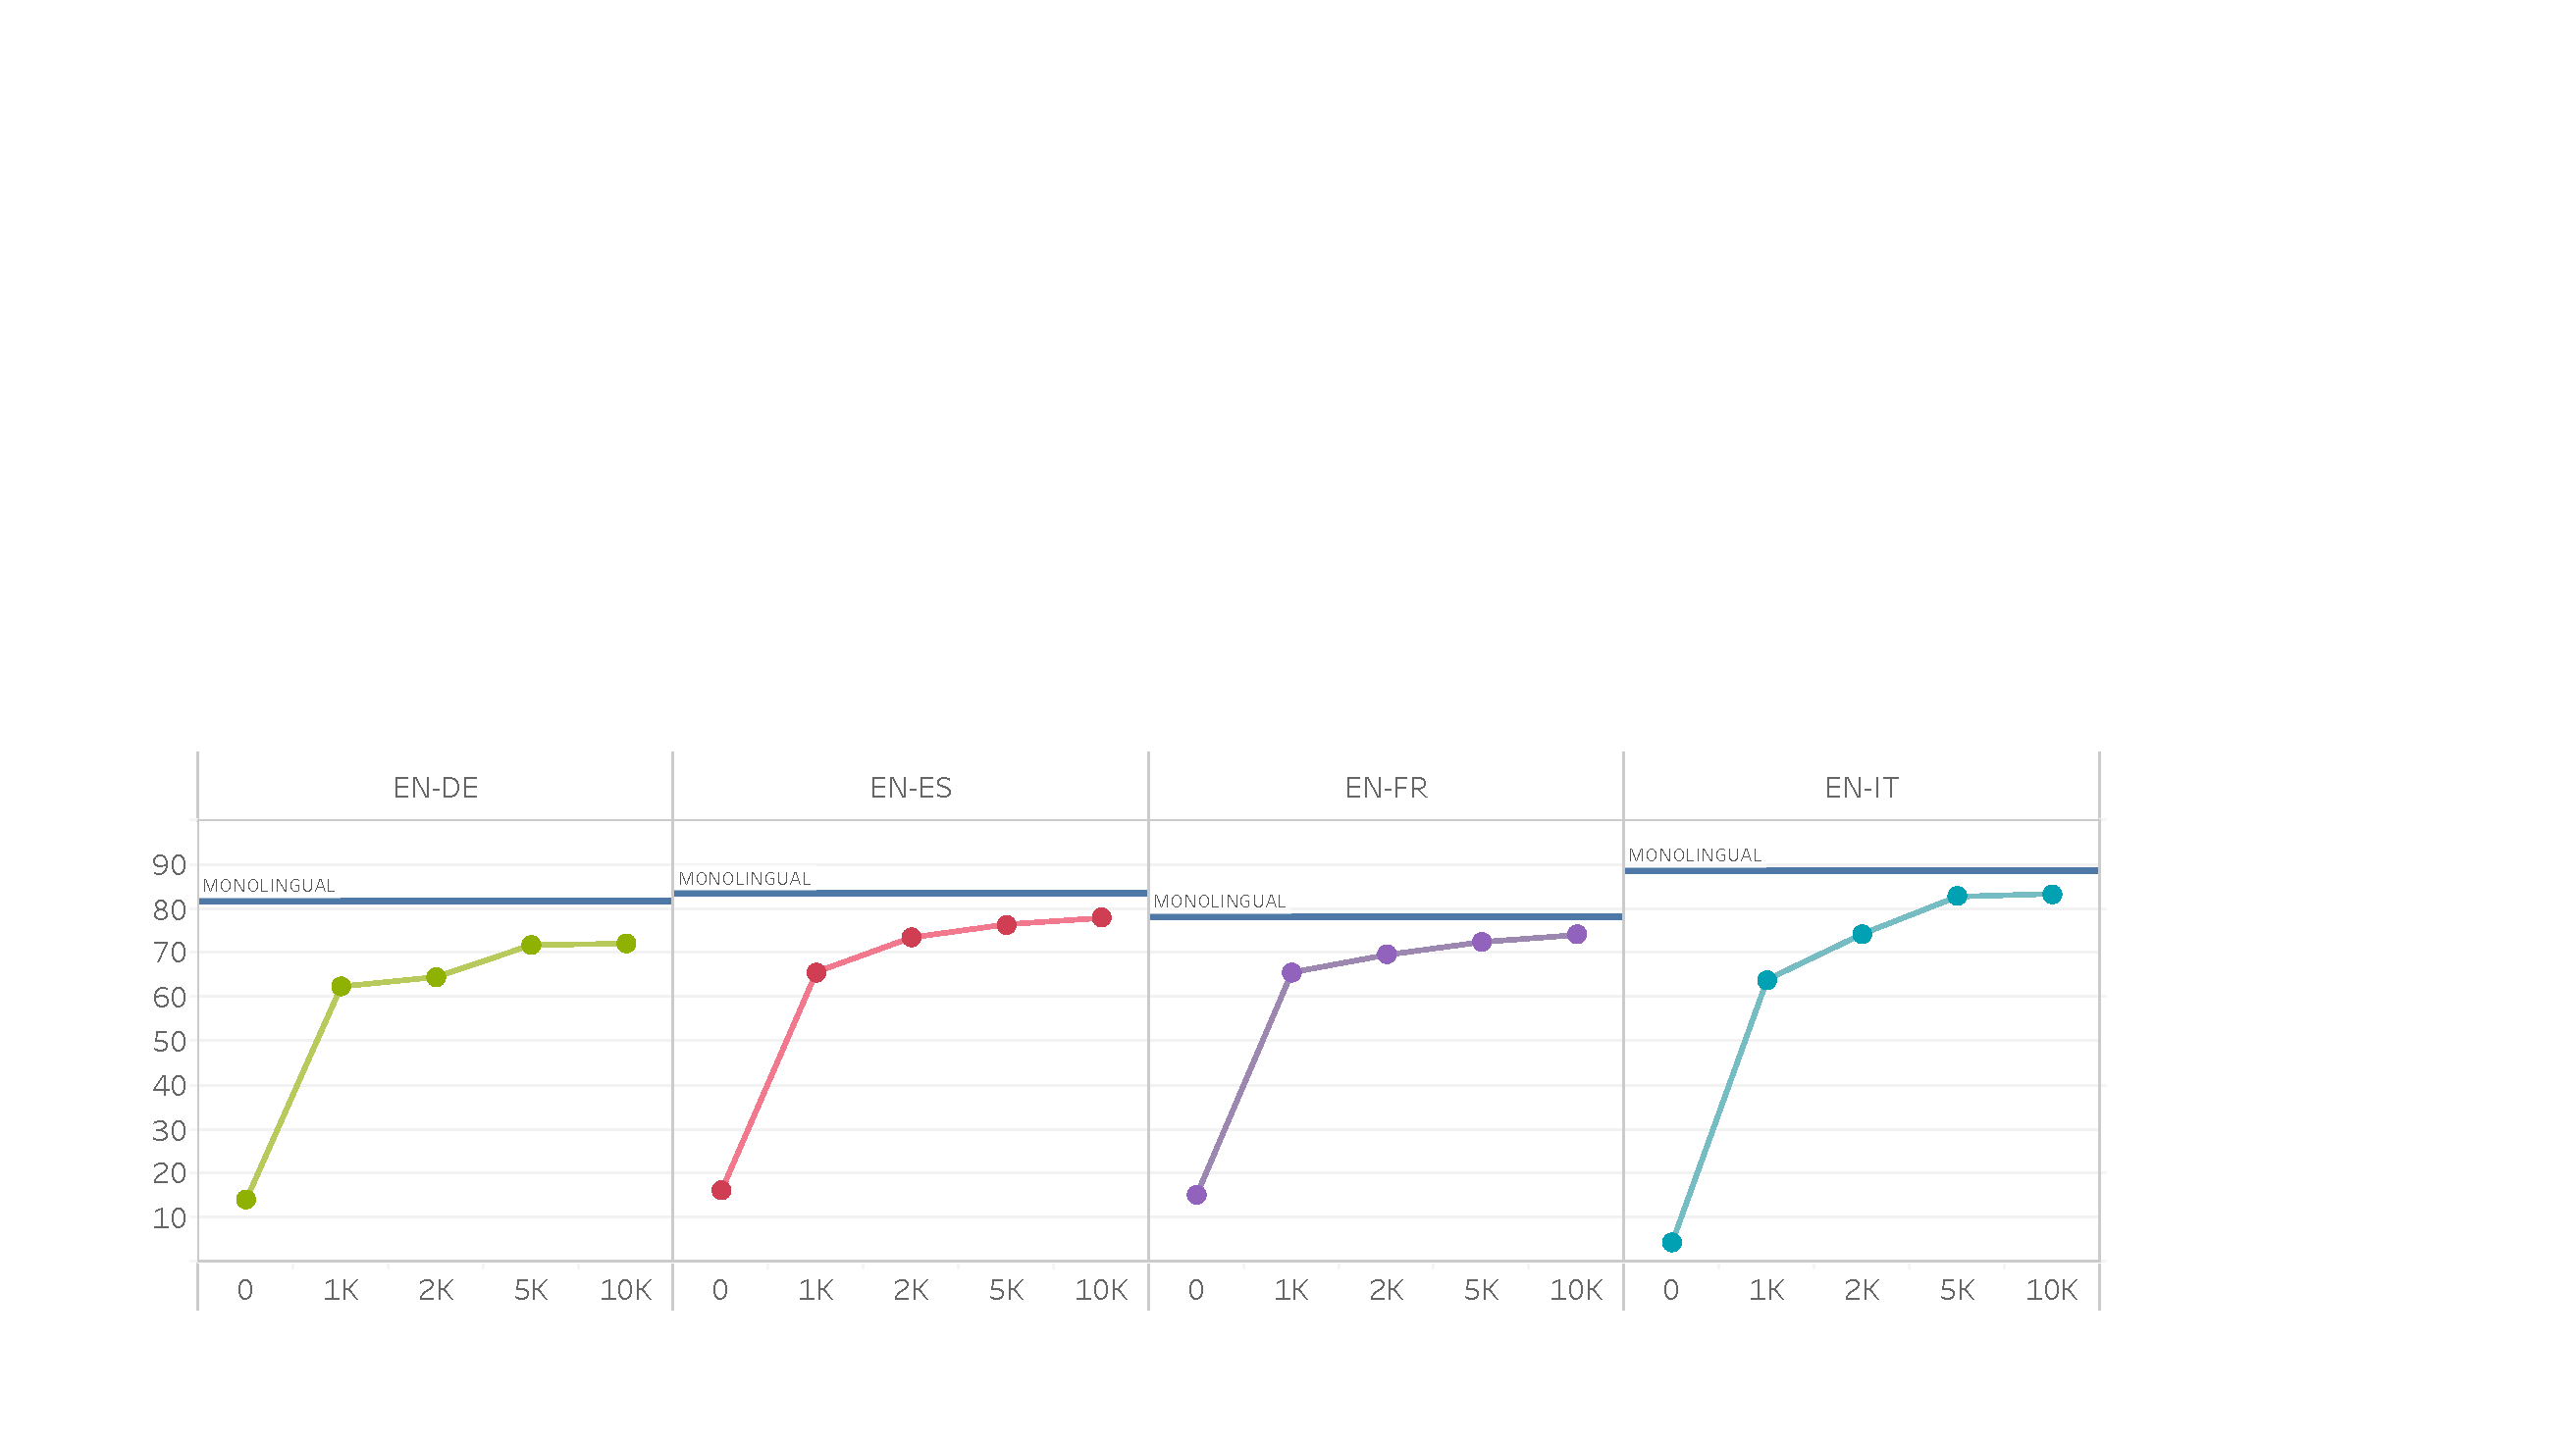
\includegraphics[width=\textwidth]{images/UnENT_color_fixed.pdf}
\caption{F1-scores for the cross-lingual transfer experiments in the \textbf{UnENT} setting. The \textsc{Monolingual} line shows the corresponding monolingual model's F1-score.}
\label{fig:UnEntF1}
\end{figure*} 

The \textbf{UnREL} is a considerably more challenging setting, we are interested in evaluating along a different dimension (question \textbf{b}): when relations are seen in the source language but not in the target language.  Figure~\ref{fig:UnREL} shows the results for the \textbf{UnREL} setup. In this case, we perform the transfer with 10K examples, and similarly to \textbf{UnENT}, the results show that it’s possible to recover a large part of the fully-supervised monolingual models’ performance, but not as much as before. This indicates that it is more challenging to transfer the ability to identify relation paraphrases and entity types through global indications (when context phrasing differs from the question in a way that is shared between relations) which \cite{levy2017zero} suggested are important for generalizing to new relations in this framework.



\begin{figure}[h!]
\centering
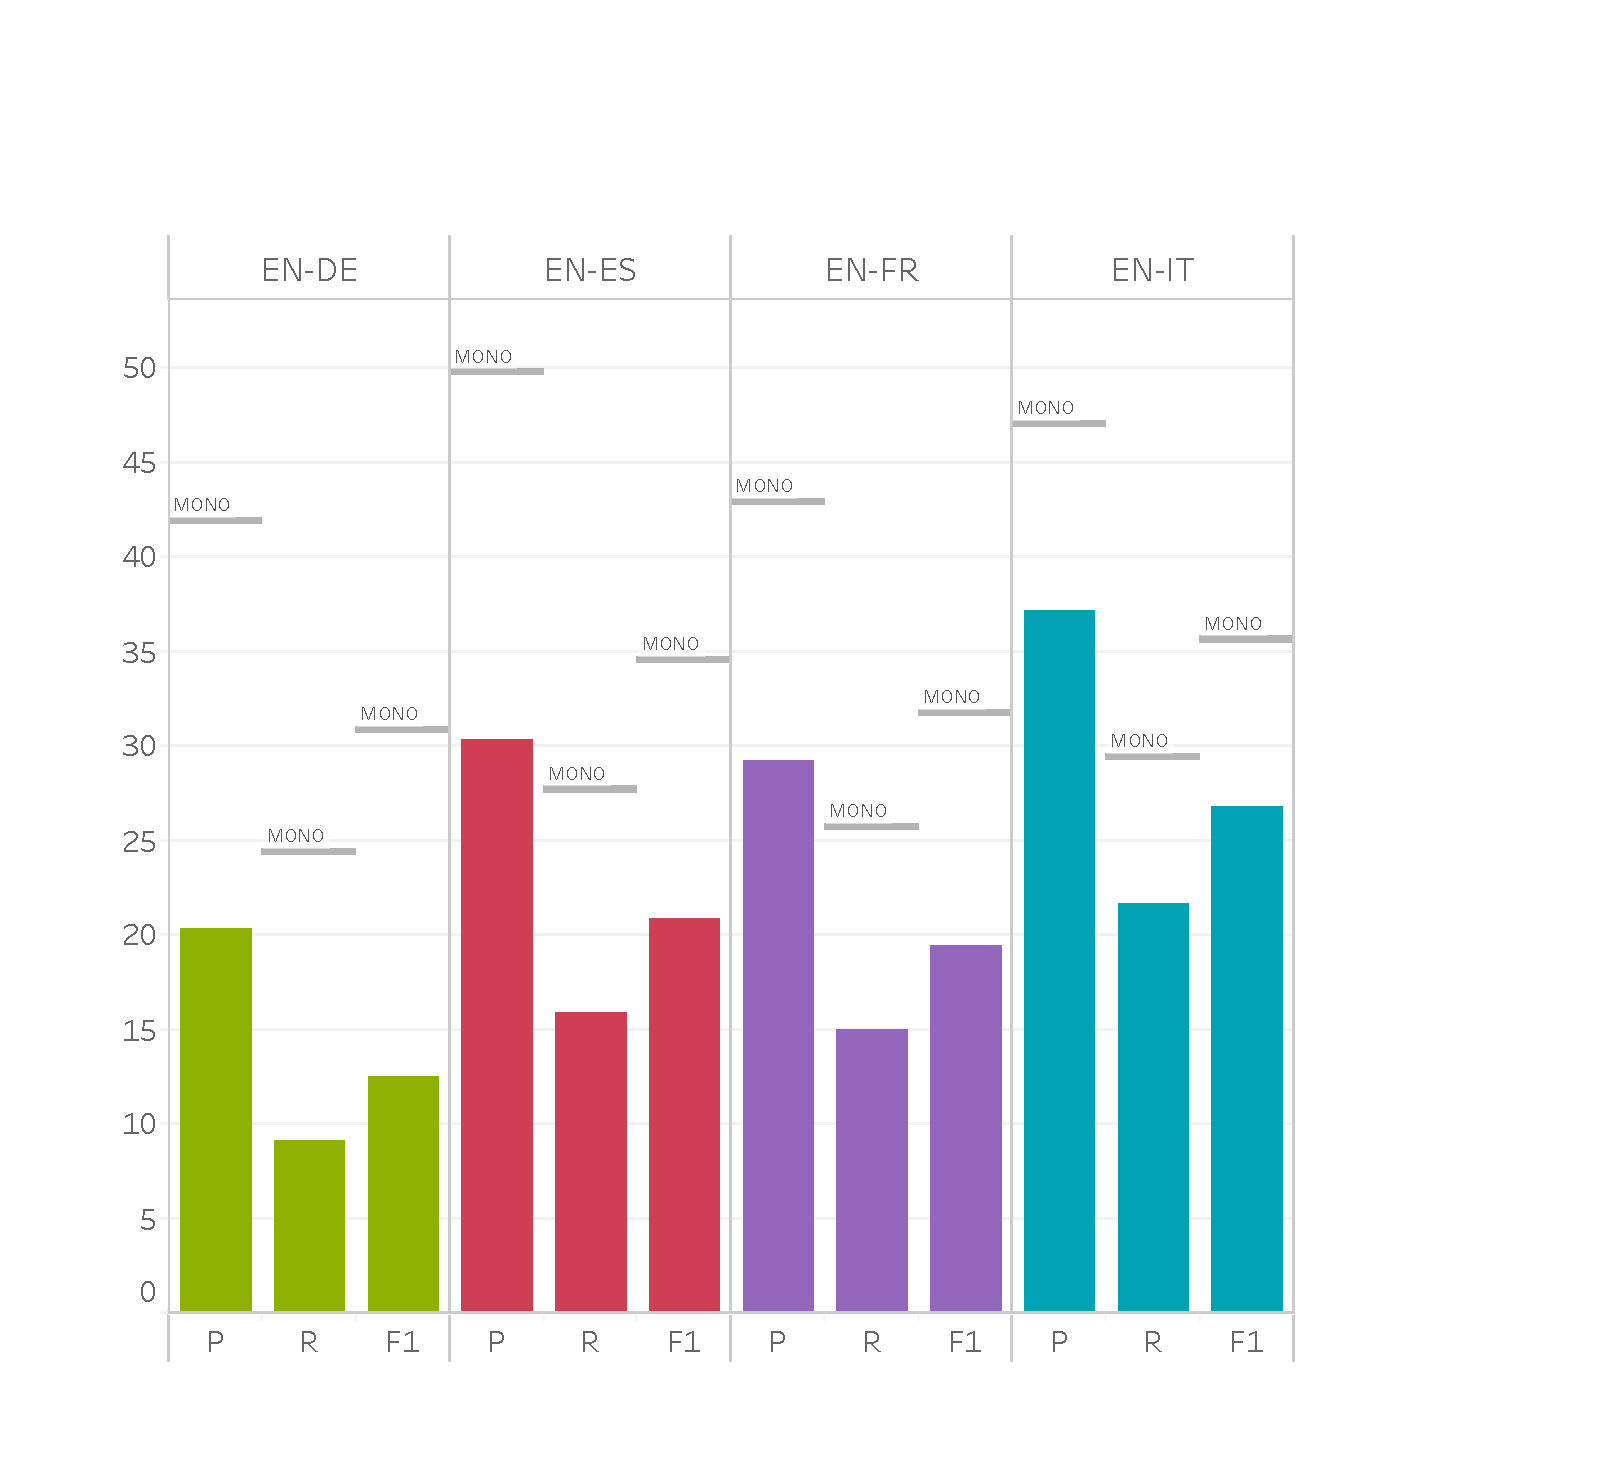
\includegraphics[width=0.6\textwidth]{images/UnREL_all_no_side_label.pdf}
\caption{Precision, Recall and F1-scores for the cross-lingual transfer experiments in \textbf{UnREL} setting. The results are the mean of 5-fold cross-validation. The \textsc{Mono} line shows the corresponding monolingual model's F1-score.}
\label{fig:UnREL}
\end{figure}


\subsection{One Model, Multiple Languages}
\paragraph{}
We now evaluate the model jointly trained on multiple languages. We are interested in exploiting the fact that KBs are better populated for different properties across different languages (question \textbf{c})
. We perform a 5-folds cross-validation, in each experiment a test set relation for a particular language is not seen in that language's training set, but may be seen in any of the other languages. This amounts to maintaining the original zero-shot setting (where a relation is not seen) monolingually, but providing supervision by allowing the models to \textit{peek across languages}.  To control for training set size we include 200K training instances per language (Multi. (S)), so that the total size of the training set is equal to that of the monolingual baseline. However, an additional benefit of multilingual training is that extra overall training data becomes available. To test the effect of that we also run an experiment where the full training set of each of the languages is employed, adding up to 5 million training examples (Multi. (L)).

In the \textbf{UnENT} setting the multilingual models trained on just 200k instances per language perform slightly below the monolingual baselines. This excludes for French where, surprisingly, the baseline performance is actually exceeded. When the full training sets of all languages are combined, the multilingual model outperforms the monolingual baselines for English, Spanish, and French and is slightly worse for German and Italian. This demonstrates that not only is it possible to utilize a single model to perform RE in multiple languages, but that the multilingual supervision signal will often lead to improvements in performance. These results are shown in the third and fourth columns of Table \ref{table:bigtable}. 

The multilingual \textbf{UnREL} model outperforms its monolingual counterparts by large margins for all languages. For many of the languages the improvements in F1-score are doubled.
This is largely in line with our premise that the natural topicality of KBs across languages can be exploited to provide cross-lingual supervision for relation extraction models. 


\begin{table}[h]
\fontsize{10}{10}\selectfont
%\begin{adjustbox}{width=\textwidth}
  \centering
  %\scriptsize
    \begin{tabular}{c|c|ccc|cc}
    \toprule
    \multirow{2}{*}{Lang.} & &  \multicolumn{3}{c|}{UnENT} & \multicolumn{2}{c}{UnREL} \\

     &  & Mono. & Multi. (S) & Multi. (L) & Mono. & Multi. \\
     \midrule
     
     \multirow{3}{*}{EN} & P  &    74.09 & 74.33 & \textbf{77.11} &    46.75 & \textbf{63.29} \\
                         & R  &    85.35 & 83.63 & \textbf{86.42} &    25.32 & \textbf{44.40} \\
                         & F1 &    79.32 & 78.71 & \textbf{81.50} &    32.78 & \textbf{51.99} \\

     \midrule
     \multirow{3}{*}{ES} & P  &    81.79 & 80.60 & \textbf{83.68} &    49.77 & \textbf{73.43} \\
                         & R  &    \textbf{85.02} & 81.47 & 83.58 &    27.69 & \textbf{62.82} \\
                         & F1 &    83.37 & 81.03 & \textbf{83.63} &    34.54 & \textbf{67.64} \\

     \midrule
     \multirow{3}{*}{IT} & P  &    \textbf{88.69} & 86.23 & 88.43 &    47.09 & \textbf{68.66} \\
                         & R  &    \textbf{88.10} & 85.64 & 86.91 &    29.45 & \textbf{55.24} \\
                         & F1 &    \textbf{88.39} & 85.93 & 87.66 &    35.62 & \textbf{61.13} \\

     \midrule
     \multirow{3}{*}{FR} & P  &    82.36 & 80.82 & \textbf{82.90} &    42.93 & \textbf{60.78} \\
                         & R  &    74.16 & 76.60 & \textbf{78.10} &    25.73 & \textbf{47.09} \\
                         & F1 &    78.05 & 78.66 & \textbf{80.43} &    31.78 & \textbf{53.06} \\

     \midrule
     \multirow{3}{*}{DE} & P  &    \textbf{75.85} & 69.88 & 73.67 &    41.94 & \textbf{43.36} \\
                         & R  &    \textbf{88.21} & 81.36 & 84.08 &    24.38 & \textbf{25.32} \\
                         & F1 &    \textbf{81.57} & 75.20 & 78.53 &    30.82 & \textbf{31.97} \\

    \bottomrule
    \end{tabular}
    %\end{adjustbox}
      \caption{Precision, Recall, and F1-score results for all languages' monolingual (Mono.) and multilingual (Multi.) models. (S) indicates the small multilingual model which was trained on 200K examples and (L) indicates the large on trained on 5 million examples.}
  \label{table:bigtable}
\end{table}


\section{Reading Comprehension Model}
\paragraph{}
To evaluate how the reading comprehension model affects the performances, we compared NAMANDA (Monolingual) with the nil-aware BiDAF~\citep{levy2017zero}. For the comparison we used their dataset, and trained both system in a monolingual fashion using GloVe embeddings. The results presented in Table~\ref{table:comparison} are in line with these presented in \citep{kundu2018namanda}, however these results are higher than when using \textbf{X-WikiRE}, this is a consequence of the differences in the datasets, the embeddings, and the training. \textbf{X-WikiRE} context are a bit longer than these in ~\cite{levy2017zero} (Table~\ref{tab:addlabel}), moreover the coverage of GloVe is higher. Also, the main difference is that in our setup we only used 5-folds instead of 10-folds, meaning that the model sees less unique relations during the training phase and is also tested on more.   


\begin{table*}[h!]
\fontsize{10}{10}\selectfont
%\begin{adjustbox}{width=\textwidth}
  \centering
  %\scriptsize
    \begin{tabular}{c|c|cc|cc}
    \toprule
    \multirow{2}{*}{Lang.} & &  \multicolumn{2}{c|}{UnENT} & \multicolumn{2}{c}{UnREL} \\

     &  &  \cite{levy2017zero} & Monolingual &  \cite{levy2017zero} & Monolingual \\
     \midrule
     
    \multirow{3}{*}{EN*} & P  & 87.66 & \textbf{90.49} & 43.61 & \textbf{56.53} \\
                         & R  & 91.32 & \textbf{94.87} & 36.45 & \textbf{44.74} \\
                         & F1 & 89.44 & \textbf{92.63} & 39.61 & \textbf{49.85} \\


    \bottomrule
    \end{tabular}
    %\end{adjustbox}
      \caption{Comparison with \cite{levy2017zero}. The models are compared on their monolingual dataset in English (EN*).}
  \label{table:comparison}
\end{table*}

